\documentclass[11pt,a4paper]{article}

% The document deliberately uses only black ink and white paper.
\usepackage[utf8]{inputenc}
\usepackage[T1]{fontenc}
\usepackage[a4paper,margin=22mm,headheight=14pt]{geometry}
\usepackage{lmodern}
\usepackage{microtype}
\usepackage{array}
\usepackage{booktabs}
\usepackage{longtable}
\usepackage{tabularx}
\usepackage{amsmath}
\usepackage{enumitem}
\usepackage{tikz}
\usetikzlibrary{positioning,arrows.meta}
\usepackage[hidelinks]{hyperref}
\usepackage{fancyhdr}
\usepackage{lastpage}

\setlength{\parindent}{0pt}
\setlength{\parskip}{6pt}
\setlist[itemize]{leftmargin=18pt,itemsep=2pt,topsep=2pt}
\setlist[enumerate]{leftmargin=20pt,itemsep=3pt,topsep=2pt}
\renewcommand{\arraystretch}{1.18}
\newcolumntype{Y}{>{\raggedright\arraybackslash}X}
\newcolumntype{L}[1]{>{\raggedright\arraybackslash}p{#1}}

\pagestyle{fancy}
\fancyhf{}
\fancyhead[L]{\textsc{ProgressPath documentation}}
\fancyhead[R]{\textsc{Current implementation}}
\fancyfoot[C]{\thepage\ / \pageref{LastPage}}
\renewcommand{\headrulewidth}{0.4pt}
\renewcommand{\footrulewidth}{0.4pt}

\newcommand{\code}[1]{\texttt{#1}}
\newcommand{\blackrule}{\rule{\linewidth}{0.6pt}}

\begin{document}

\thispagestyle{empty}
\vspace*{25mm}
{\Huge\bfseries ProgressPath}\par
\vspace{3mm}
{\Large Educational progress tracker}\par
\vspace{10mm}
\blackrule
\vspace{5mm}
{\large Project documentation}\par
\vspace{2mm}
JavaFX \textbullet{} SQLite \textbullet{} MVC\par
\vspace{12mm}
\begin{tabular}{@{}ll@{}}
  Documentation date: & 10 September 2026\\
  Implementation: & Minimal MVC desktop application\\
  Build: & Maven, Java 17 release, JavaFX 21\\
  Persistence: & SQLite database in \code{data/progresspath.db}
\end{tabular}
\vfill
\blackrule
\vspace{3mm}
\small This document describes the source currently in \code{ProgressPath}. It is intentionally monochrome for reliable printing and review.
\newpage

\tableofcontents
\newpage

\section{Overview}

ProgressPath is a local desktop application for planning academic work and checking whether actual progress follows a target schedule. A student can create study plans, organise courses and weighted chapters, record progress history, manage assignments, run focus sessions, and inspect plan-level and course-level risk summaries.

The current implementation is deliberately small but complete enough to demonstrate the main workflows. The JavaFX view is a single shell with eight tabs. The controller coordinates user actions, the model facade owns validation and calculations, repositories isolate SQL, and SQLite stores data across restarts.

\section{Scope and screens}

The current view is implemented in \code{main.fxml} and controlled by \code{MainController}. The screens and their responsibilities are:

\begin{longtable}{@{}L{0.20\linewidth}L{0.72\linewidth}@{}}
\toprule
\textbf{Screen} & \textbf{Current features}\\
\midrule
\endhead
Dashboard & Select an active plan; show actual and expected progress, status, overdue assignment count, course-risk table, and the next five active assignments.\\
Study plans & Create and edit plans, choose start and end dates, archive or restore a plan, and delete a plan with its dependent data.\\
Plan details & Select a plan, create or edit courses, create or edit chapters, assign chapter weights, set target dates, and review the course weight total.\\
Progress & Select a calculation strategy and course, update a chapter percentage, view progress history, and compare actual versus expected progress.\\
Assignments & Create or edit an assignment with course, title, description, due date, priority, and status; delete selected assignments.\\
Focus & Choose a course and optional chapter, start/pause/resume/complete/cancel a timer, add a note, and view saved sessions.\\
Analytics & Choose a plan and date range; show actual progress, expected progress, completed assignments, focus time, and an at-risk course report.\\
Assistant & Select an active plan, ask a study question, and receive an asynchronous Gemini Flash response based on a compact plan snapshot. The assistant does not edit stored data.\\
\bottomrule
\end{longtable}

Charts, system notifications, and full-text assignment search are intentionally outside this minimal slice and are suitable future extensions.

\section{Architecture}

The application follows a compact Model--View--Controller flow:

\begin{center}
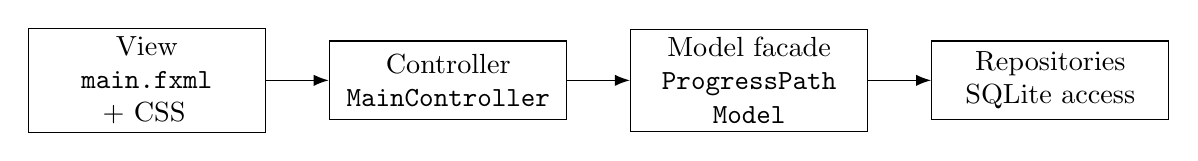
\begin{tikzpicture}[node distance=9mm and 8mm,
  box/.style={draw=black,rectangle,minimum height=10mm,text width=28mm,align=center,inner sep=3pt},
  arrow/.style={-Latex,draw=black,line width=0.55pt}]
  \node[box] (view) {View\\\code{main.fxml} + CSS};
  \node[box,right=of view] (controller) {Controller\\\code{MainController}};
  \node[box,right=of controller] (model) {Model facade\\\code{ProgressPath}\\\code{Model}};
  \node[box,right=of model] (repo) {Repositories\\SQLite access};
  \draw[arrow] (view) -- (controller);
  \draw[arrow] (controller) -- (model);
  \draw[arrow] (model) -- (repo);
\end{tikzpicture}
\end{center}

\begin{itemize}
  \item \textbf{View:} FXML declares controls and event names; CSS supplies the monochrome/blue application styling. The PDF documents the logic, not the screen colours.
  \item \textbf{Controller:} named handlers validate form-level concerns, call the model, and refresh tables and choices. It contains no SQL.
  \item \textbf{Model facade:} \code{ProgressPathModel} exposes plan, progress, assignment, focus, and analytics operations, validates domain rules, and notifies observers after mutations.
  \item \textbf{Persistence:} \code{DatabaseManager} opens SQLite connections with foreign keys enabled; repositories map rows to immutable Java records.
  \item \textbf{Headless seeding:} \code{SeedRunner} initializes the schema and invokes \code{DatabaseSeeder.seedDemoData()} without launching JavaFX.
  \item \textbf{AI provider:} the controller calls the \code{AssistantProvider} boundary; \code{GeminiFlashAssistantProvider} performs the network request without coupling Gemini code to JavaFX or SQLite.
\end{itemize}

\section{AI assistant integration}

The Assistant tab is an optional study-support screen. It uses the selected active plan to provide practical explanations, prioritisation suggestions, and short study plans. Existing progress calculations and database operations remain deterministic Java code; Gemini is used only to interpret the supplied snapshot and write guidance.

\subsection{Request flow}

\begin{enumerate}
  \item The student selects an active study plan and enters a question.
  \item The controller builds a compact context containing plan dates, actual and expected progress, courses, chapter progress/weights/targets, active assignments, and completed focus time.
  \item A JavaFX \code{Task} calls \code{AssistantProvider} on a daemon worker thread so the interface remains responsive.
  \item \code{GeminiFlashAssistantProvider} sends a \code{generateContent} request to the configured Flash model and returns the first text response.
  \item The controller displays the answer or a clear configuration/network error; no AI response is written to SQLite.
\end{enumerate}

\subsection{Configuration and boundaries}

The local project includes \code{.env.example}. Copy it to \code{.env} and set \code{GEMINI\_API\_KEY}; \code{.env} is ignored by Git. The provider accepts the documented \code{GOOGLE\_API\_KEY} or \code{GEMINI\_API\_KEY} environment variables (\code{GOOGLE\_API\_KEY} takes precedence), or the \code{-Dgoogle.api.key} / \code{-Dgemini.api.key} JVM properties. \code{GEMINI\_MODEL} and \code{GEMINI\_TIMEOUT\_SECONDS} are optional overrides. The default model is \code{gemini-3.8-flash} and the default request timeout is 45 seconds.

The HTTP client follows the Gemini REST \code{models.generateContent} shape. It uses the \code{x-goog-api-key} header for authentication, keeping the key out of the request URL, and posts JSON containing a system instruction, one user content part, and a 512-token output limit.

If Google returns HTTP 403 with ``Your project has been denied access'', the failure is project/key policy rather than application JSON. Create a new authorization key in an accessible Google AI Studio project, restrict it to the Gemini API, and replace the local value. The desktop client cannot override a denied project.

The app deliberately sends only the selected plan snapshot and the current question. It does not send the full database, prior conversation, or API key in the request body. For a distributed release, the provider call should move behind a server-side proxy so a key is not shipped in a desktop binary. The current minimal screen requires network access, does not persist chat history, and cannot guarantee that generated advice is correct; students should verify important academic decisions.

\subsection{Changes in this revision}

This revision adds the eighth, Assistant tab; the provider interface, Gemini Flash HTTP client, compact context builder, asynchronous JavaFX request handling, local \code{.env} loading, and the tracked \code{.env.example} template. Existing plan, course, progress, assignment, focus, analytics, persistence, and test workflows remain unchanged.

\section{Database design}

\subsection{Entity relationship view}

The database has six application tables. A plan owns courses; a course owns chapters and assignments; a chapter owns progress history; and focus sessions belong to a course with an optional chapter link.

\begin{center}
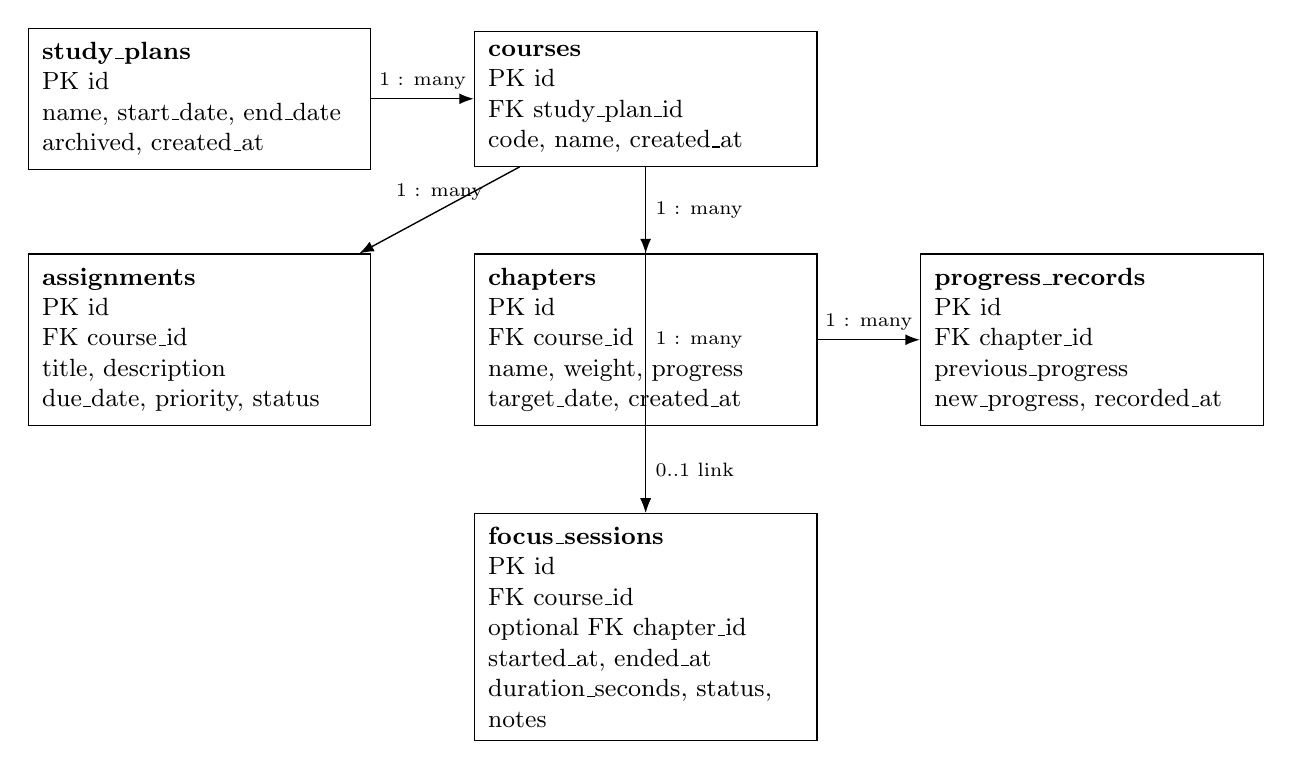
\begin{tikzpicture}[node distance=11mm and 13mm,
  entity/.style={draw=black,rectangle,align=left,text width=40mm,inner sep=5pt,font=\small},
  rel/.style={-Latex,draw=black,line width=0.5pt}]
  \node[entity] (plan) {\textbf{study\_plans}\\PK id\\name, start\_date, end\_date\\archived, created\_at};
  \node[entity,right=of plan] (course) {\textbf{courses}\\PK id\\FK study\_plan\_id\\code, name, created\_at};
  \node[entity,below=of course] (chapter) {\textbf{chapters}\\PK id\\FK course\_id\\name, weight, progress\\target\_date, created\_at};
  \node[entity,left=of chapter] (assignment) {\textbf{assignments}\\PK id\\FK course\_id\\title, description\\due\_date, priority, status};
  \node[entity,right=of chapter] (history) {\textbf{progress\_records}\\PK id\\FK chapter\_id\\previous\_progress\\new\_progress, recorded\_at};
  \node[entity,below=of chapter] (focus) {\textbf{focus\_sessions}\\PK id\\FK course\_id\\optional FK chapter\_id\\started\_at, ended\_at\\duration\_seconds, status, notes};
  \draw[rel] (plan) -- node[above,font=\scriptsize]{1 : many} (course);
  \draw[rel] (course) -- node[right,font=\scriptsize]{1 : many} (chapter);
  \draw[rel] (course) -- node[above,font=\scriptsize]{1 : many} (assignment);
  \draw[rel] (chapter) -- node[above,font=\scriptsize]{1 : many} (history);
  \draw[rel] (course) -- node[right,font=\scriptsize]{1 : many} (focus);
  \draw[rel] (chapter) -- node[right,font=\scriptsize]{0..1 link} (focus);
\end{tikzpicture}
\end{center}

\subsection{Tables and constraints}

The schema is created idempotently by \code{DatabaseSeeder.initialize()}. Existing databases receive an \code{archived} column migration when needed.

\small
\begin{longtable}{@{}L{0.19\linewidth}L{0.40\linewidth}L{0.31\linewidth}@{}}
\toprule
\textbf{Table} & \textbf{Columns} & \textbf{Keys and rules}\\
\midrule
\endhead
\code{study\_plans} & \code{id}, \code{name}, \code{start\_date}, \code{end\_date}, \code{archived}, \code{created\_at} & Primary key \code{id}; unique non-null \code{name}; \code{archived} is 0 or 1; end date must be after start date.\\
\code{courses} & \code{id}, \code{study\_plan\_id}, \code{code}, \code{name}, \code{created\_at} & Primary key; plan foreign key with \code{ON DELETE CASCADE}; unique \code{(study\_plan\_id, code)}.\\
\code{chapters} & \code{id}, \code{course\_id}, \code{name}, \code{weight}, \code{progress}, \code{target\_date}, \code{created\_at} & Course foreign key with cascade; unique \code{(course\_id, name)}; weight is greater than 0 and at most 100; progress is 0--100.\\
\code{progress\_records} & \code{id}, \code{chapter\_id}, \code{previous\_progress}, \code{new\_progress}, \code{recorded\_at} & Chapter foreign key with cascade; both progress values are 0--100; indexed by \code{chapter\_id}.\\
\code{assignments} & \code{id}, \code{course\_id}, \code{title}, \code{description}, \code{due\_date}, \code{priority}, \code{status} & Course foreign key with cascade; priority is \code{LOW}, \code{MEDIUM}, or \code{HIGH}; status is \code{PENDING}, \code{IN\_PROGRESS}, \code{COMPLETED}, or \code{CANCELLED}; indexed by due date.\\
\code{focus\_sessions} & \code{id}, \code{course\_id}, nullable \code{chapter\_id}, \code{started\_at}, \code{ended\_at}, \code{duration\_seconds}, \code{status}, \code{notes} & Course foreign key with cascade; optional chapter foreign key with \code{ON DELETE SET NULL}; duration is non-negative; status is \code{COMPLETED} or \code{CANCELLED}; indexed by start time.\\
\bottomrule
\end{longtable}
\normalsize

\subsection{Persistence rules}

\begin{itemize}
  \item Every connection executes \code{PRAGMA foreign\_keys = ON} and sets a three-second busy timeout.
  \item Domain validation supplements SQLite checks: plan dates are checked in the model, chapter weights are checked against the other chapters in the course, and text fields are trimmed and required where appropriate.
  \item Deleting a plan cascades to courses, chapters, assignments, focus sessions, and progress records through the foreign-key chain.
  \item The demo seeder uses one transaction, rolls back on failure, and returns a \code{SeedingReport}. If any plan already exists, it inserts nothing.
  \item Current demo data contains 11 study plans, 22 courses, 61 chapters, 30 progress records, 43 assignments, and 30 focus sessions.
\end{itemize}

\section{Design patterns used}

The following patterns are present in the current source. Each is used for a concrete separation or extension point rather than only for demonstration.

\small
\begin{longtable}{@{}L{0.18\linewidth}L{0.31\linewidth}L{0.42\linewidth}@{}}
\toprule
\textbf{Pattern} & \textbf{Implementation} & \textbf{Why it is used}\\
\midrule
\endhead
MVC & \code{main.fxml} (View), \code{MainController} (Controller), \code{ProgressPathModel} and records (Model) & Separates JavaFX event wiring from validation, calculations, and persistence. A screen can change without moving SQL or business rules into the view.\\
Repository & \code{StudyPlanRepository}, \code{CourseRepository}, \code{ChapterRepository}, \code{AssignmentRepository}, \code{FocusSessionRepository}, \code{ProgressRecordRepository} & Encapsulates SQL and row mapping. The model depends on simple domain operations instead of database statements, which keeps tests and a future storage replacement manageable.\\
Strategy & \code{ProgressCalculationStrategy}, weighted/equal policy classes, selected through \code{ProgressCalculator} & Makes the progress policy interchangeable. Weighted progress respects chapter weights; equal progress treats every chapter equally without changing the controller or model workflow.\\
State & \code{FocusSessionState} with Ready, Running, Paused, Completed, and Cancelled states; \code{FocusTimer} is the context & Keeps valid timer transitions next to the state that owns them. Invalid actions fail clearly, while timing details stay out of the JavaFX controller.\\
Observer & \code{ModelChangeListener}, \code{ModelChangeType}, and the controller subscription & A completed mutation notifies the interested UI. Tables, choices, dashboard metrics, and analytics refresh together without each editor knowing the internals of the other screens.\\
Provider Strategy & \code{AssistantProvider} with \code{GeminiFlashAssistantProvider} & Isolates the AI vendor and HTTP details from the controller. A second provider or a local test double can be added without changing the Assistant screen.\\
\bottomrule
\end{longtable}
\normalsize

\section{Patterns considered but skipped}

These patterns are reasonable future options, but adding them to the current minimal slice would increase indirection without solving an active problem.

\small
\begin{longtable}{@{}L{0.20\linewidth}L{0.38\linewidth}L{0.33\linewidth}@{}}
\toprule
\textbf{Pattern} & \textbf{Potential use} & \textbf{Reason it is skipped now}\\
\midrule
\endhead
Factory Method / Abstract Factory & Construct different report objects such as weekly, monthly, and risk reports. & Analytics currently returns one parameterised \code{AnalyticsSummary}; separate report products would be premature until report formats diverge.\\
Singleton & Make the database manager or application model globally accessible. & Global state would make isolated tests and multiple database paths harder. Dependencies are passed explicitly instead.\\
Command & Represent every button action as an object for undo, redo, or a work queue. & The current UI has immediate CRUD and timer actions, with no undo history or background command queue.\\
Decorator & Add optional cross-cutting behaviour such as logging, caching, or notifications around services. & The application has one local persistence path and no independent service implementations that need runtime composition.\\
Adapter & Wrap a second database, remote API, or external calendar behind the same interface. & SQLite is the only storage integration in this release; a wrapper would add code without a second incompatible API.\\
Event bus & Route many event types between numerous independent modules. & There are only a few screens and one model owner, so the small typed Observer interface is easier to trace and test.\\
\bottomrule
\end{longtable}
\normalsize

\section{Core workflows and calculations}

\subsection{Plan and progress workflow}

\begin{enumerate}
  \item Create a plan with a valid date range.
  \item Add courses and chapters. The model validates required text, target dates, and the course's total chapter weight.
  \item Choose weighted or equal chapter progress on the Progress screen.
  \item Save a percentage for a chapter. The old value, new value, and timestamp are written to \code{progress\_records} before the UI is notified.
  \item The dashboard and analytics calculate expected progress from the plan start and each chapter target (or plan end when no target exists), then classify the variance as Ahead, On track, Slightly behind, or Significantly behind.
\end{enumerate}

For weighted progress:
\[
  \text{progress} = \frac{\sum(\text{chapter progress}\times\text{chapter weight})}
  {\sum(\text{chapter weight})}.
\]
Equal progress averages the chapter percentages. Both policies return zero when there are no chapters.

\subsection{Assignment workflow}

Assignments are linked to courses and ordered by due date, priority, and id. Overdue means the due date is before the selected day and the status is neither Completed nor Cancelled. The dashboard shows the first five active assignments; Analytics counts completed and overdue work for its selected date range.

\subsection{Focus workflow}

\code{FocusTimer.start()} moves Ready to Running. Running may pause, complete, or cancel; Paused may resume, complete, or cancel. Completing or cancelling records elapsed seconds, timestamps, status, and notes in \code{focus\_sessions}. The controller uses a JavaFX timeline only to refresh the displayed clock; state transition rules remain in the State objects.

\section{Build, seed, and test}

Run these commands from the \code{ProgressPath} directory:

\begin{verbatim}
mvn test
mvn javafx:run
\end{verbatim}

The application creates \code{data/progresspath.db} automatically. To load the current demonstration dataset:

Before using the Assistant tab, copy \code{.env.example} to \code{.env} and set \code{GOOGLE\_API\_KEY} or \code{GEMINI\_API\_KEY}. The application reads this file itself; Maven does not need a dotenv plugin. Never commit the resulting \code{.env} file.

\begin{verbatim}
mvn -q -DskipTests package
mvn -q exec:java -Dexec.mainClass=com.progresspath.app.SeedRunner
\end{verbatim}

The seeder is safe to rerun: it reports \code{already\_seeded=true} and inserts zero rows when the database already contains a plan. The current automated suite covers weighted and equal progress, persistence and validation, and the focus State lifecycle.

\section{Known limits and next steps}

The implementation is intentionally a minimal application. The following items are documented rather than hidden:

\begin{itemize}
  \item Advanced assignment search and multi-field filtering are not in the current FXML.
  \item Analytics is tabular; chart components and exportable reports are future work.
  \item There is no operating-system reminder or notification service.
  \item Focus sessions are stored only when completed or cancelled; crash recovery is not yet persisted as an open-session record.
  \item Repository operations are intentionally straightforward; larger deployments could add transactions around multi-step plan setup and a service layer between the model facade and repositories.
  \item The Assistant tab depends on a configured Gemini key and network access. Responses are not stored, streamed, or used to mutate plans, courses, assignments, or progress.
\end{itemize}

\section{Source map}

The following locations are relative to \code{src/main/java/com/progresspath} unless noted otherwise.

\begin{tabularx}{\linewidth}{@{}L{0.26\linewidth}Y@{}}
\toprule
\textbf{Location} & \textbf{Responsibility}\\
\midrule
\code{app/} & JavaFX entry point and headless demo seeder.\\
\code{controller/} & FXML controller and screen event coordination.\\
\code{model/} & Immutable records, model facade, analytics values, and Observer event types.\\
\code{persistence/} & SQLite connection, schema/migration/seeding, and repositories.\\
\code{progress/} & Strategy interface and progress policies.\\
\code{focus/} & Focus timer context and State implementations.\\
\code{ai/} & Assistant provider boundary, Gemini Flash HTTP client, local configuration, and narrow response parsing.\\
\code{resources/fxml} & Eight-tab JavaFX View in \code{main.fxml}.\\
\code{resources/css} & Application styling in \code{progresspath.css}.\\
\code{src/test/java} & Unit tests for progress, persistence/validation, and focus states.\\
\bottomrule
\end{tabularx}

\vfill
\noindent\rule{\linewidth}{0.6pt}\par
{\small\textit{ProgressPath documentation -- monochrome edition.}\par}

\end{document}
